\chapter{Technical background}\label{chap:background}

Before describing pruning and random structures, we must know how RNNs and their different variants, namely LSTM and GRU, operate. Therefore, in this section, we provide a detailed explanation of RNNs, LSTM, and GRU.

To properly understand how RNNs operate, we must understand how a perceptron, a building block of neural networks, works.

% --------------------------------------------------------------------------------------------
% ---------------------------------------- PERCEPTRON ----------------------------------------
% --------------------------------------------------------------------------------------------

\section{Perceptron}\label{section:perceptron}

A perceptron, also known as a Single Layer Perceptron (SLP), is a single layer neural network developed by F. Rosenblatt in \cite{Rosenblatt}, inspired by \cite{mcculloch}. It is a linear classifier that accepts multiple binary inputs and returns a single binary output.

\begin{figure}[h]
	\centering
	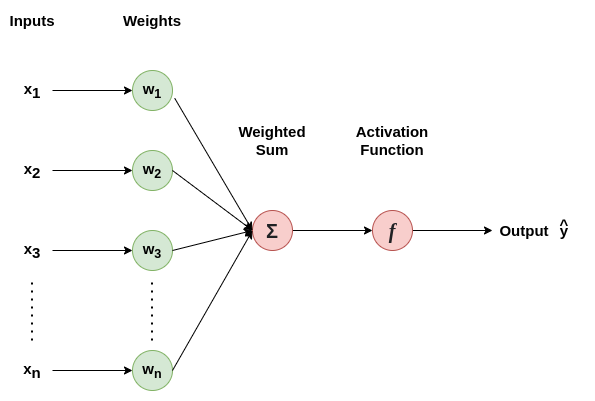
\includegraphics[width=0.7\linewidth]{images/background/perceptron.png}
	\caption[Single Layer Perceptron]%
	{\textbf{Single Layer Perceptron} with binary inputs $x_1, x_2, x_3, ..., x_n$ and its corresponding weights $w_1, w_2, w_3, ..., w_n$.}
	\label{fig:perceptron}
\end{figure}

As shown in the above figure, a perceptron consists of four main parts, inputs, weights, weighted sum, and an activation function. A perceptron works by following these simple steps:

\begin{enumerate}
    \item Multiply each input $x$ with its corresponding weight $w$.
    \item Get a value for the weighted sum by adding all the multiplied values together.
        \begin{equation}
        \label{eqn:weighted_sum}
            weighted\; sum = \sum_{i=1}^{n}w_i.x_i
        \end{equation}
    \item Apply this weighted sum to a activation function to generate the output $\hat{y}$.
\end{enumerate}

An activation function is a significant part of a perceptron. It transforms the input of the node into the output for that node. It ensures the output value is mapped between (0, 1) or (-1, 1). Rectified Linear Unit (ReLU), Hyperbolic Tangent (Tanh) are two of the popular nonlinear activation functions explained later in the following section.

\subsection{Nonlinearity (Nonlinear Activation function)}\label{subsection:nonlinearity}

A nonlinearity, as the name suggests, is used when it is not possible to produce an output for any unit using a linear function. Concerning neural networks, three of the most widely used nonlinearities are, ReLU, Sigmoid, Tanh \cite{nonlin}.

\subsubsection{ReLU}\label{subsubsection:relu}

A \textit{Rectified Linear Unit} is a nonlinear activation function mathematically defined as:

\begin{equation}
    \label{eqn:relu}
    y = max(0, x)
\end{equation}

As per the above equation, for a given input $x$, if the value of $x$ is less than $0$, it returns $0$, otherwise $x$.

The following figure shows the line plot of the ReLU activation function.

\begin{figure}[h]
    \centering
    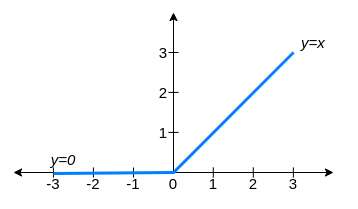
\includegraphics[width=0.5\linewidth]{images/background/relu.png}
    \caption[Rectified Linear Unit]{Line plot of ReLU activation function}
    \label{fig:relu}
\end{figure}

For any given positive input, the derivative of ReLU simply returns 1. This eliminates the need to perform computationally expensive exponentials and divisions, as required by other activation functions such as the Sigmoid activation function.

\subsubsection{Sigmoid}\label{subsubsection:sigmoid}

The \textit{Sigmoid} activation function, unlike ReLU, is mainly used in \textit{Feedforward Neural Networks}. This activation function returns a value between $0$ and $1$. The following figure shows the line plot of the Sigmoid activation function.

\begin{figure}[h]
    \centering
    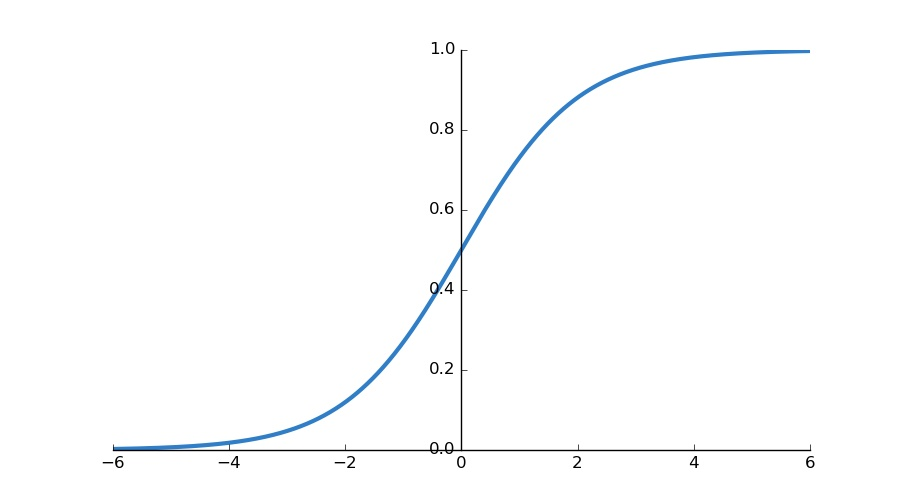
\includegraphics[width=0.7\linewidth]{images/background/sigmoid.jpg}
    \caption[Sigmoid activation function]{Line plot of Sigmoid activation function \cite{sigmoid}}
    \label{fig:sigmoid}
\end{figure}

For a given input $x$, the Sigmoid activation is mathematically written as:

\begin{equation}
    \label{eqn:sigmoid}
    S(x) = \frac{1}{1 + e^{-x}}
\end{equation}

As mention by Nwankpa et al. in \cite{activation}, this activation function has many drawbacks, including gradient saturation and slow convergence. Some of these shortcomings are possible to avoid using other forms of activation functions such as \textit{hyperbolic tangent}.

\subsubsection{Tanh}\label{subsubsection:tanh}

Tanh, short for \textit{hyperbolic tangent} is an activation function with a value range between $-1$ to $1$, making it a zero-centered activation function. The following figure shows the line plot of the Tanh activation function.

\begin{figure}[h]
    \centering
    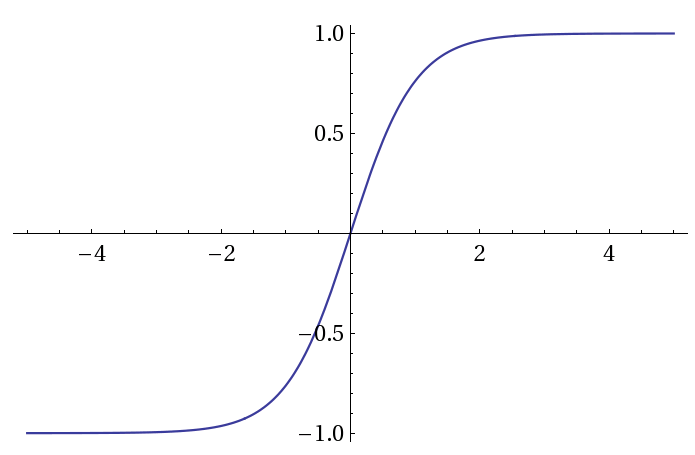
\includegraphics[width=0.6\linewidth]{images/background/tanh.png}
    \caption[Tanh activation function]{Line plot of Tanh activation function \cite{tanh}}
    \label{fig:tanh}
\end{figure}

For a given input $x$, the Tanh activation is mathematically written as:

\begin{equation}
    \label{eqn:tanh}
    tanh(x) = \frac{e^{x} - e^{-x}}{e^{x} + e^{-x}}
\end{equation}

Although compared to the Sigmoid activation function, Tanh has better performance during training \cite{tanh_1, tanh_2}, it suffers from the vanishing gradient problem.

The output from a nonlinear activation function is not a perfect match to the actual target. For this reason, it is necessary to optimize weight values such that the difference between the actual target and the final output is the smallest, which is done by a process called gradient descent.

\subsection{Batch Gradient Descent}\label{subsection:bgd}

A perceptron has fixed input and output, meaning we can only modify and improve weights to minimize errors. An error function $E$ returns the deviation of predicted outcome $\hat{y}$ from the actual one $y$ as sum of squared errors:

\begin{equation}
    \label{eq:error_func}
    E(w) = \frac{1}{2} \sum_{i=1}^{n}(\hat{y}^{(i)} - y^{(i)})^2
\end{equation}

Weights are then updated using this error function as:

\begin{equation}
    \label{eq:weight_update}
    w \coloneqq w - \eta \nabla E(\text{w})
\end{equation}

where $\eta$ is the learning rate and $\nabla E(\text{w})$ is partial derivative of the cost function, computed for each weight in the weight vector as:

\begin{equation}
    \label{eq:part_der}
    \nabla E(\text{w}) = \frac{\partial E(\text{w})}{\partial w_j}
\end{equation}

By substituting the value of $E(\text{w})$ from equation \ref{eq:error_func} in above equation, we can derive $\nabla E(\text{w})$, as shown by \cite{perc_eq}, as:

\begin{align}
    \nabla E(\text{w}) &= \frac{\partial}{\partial w_j}\frac{1}{2} \sum_{i=1}^{n}(\hat{y}^{(i)} - y^{(i)})^2 \nonumber \\
                       &= \frac{1}{2} \sum_{i=1}^{n}\frac{\partial}{\partial w_j}(\hat{y}^{(i)} - y^{(i)})^2 \nonumber \\
                       &= \frac{1}{2} \sum_{i=1}^{n}2(\hat{y}^{(i)} - y^{(i)})\frac{\partial}{\partial w_j}(\hat{y}^{(i)} - y^{(i)}) \nonumber \\
                       &= \sum_{i=1}^{n}(\hat{y}^{(i)} - y^{(i)}) \frac{\partial}{\partial w_j}(\hat{y}^{(i)} - \sum_{j}w_{j}.x_{j}^{(i)}) \nonumber \\
                       &= \sum_{i=1}^{n}(\hat{y}^{(i)} - y^{(i)})(-x_{j}^{(i)}) \label{eq:part_derived}
\end{align}

By substituting the value from equations \ref{eq:part_derived} in \ref{eq:weight_update}, we can re-write the weight update formula as:

\begin{equation}
    w \coloneqq w + \eta \sum_{i=1}^{n}(\hat{y}^{(i)} - y^{(i)})(x_{j}^{(i)})
\end{equation}

This approach for updating weights is known as Batch Gradient Descent because each sample in the training set is considered at each step of weights update. Repetition of these training and weights update steps is necessary to obtain convergence.

An SLP has no hidden layers. By adding one or more hidden layers, we can generate a Multi-Layer Perceptron (MLP), also known as an Artificial Neural Network (ANN) or simply, a Neural Network.

% ------------------------------------------------------------------------------------------------------------
% ---------------------------------------- ARTIFICIAL NEURAL NETWORKS ----------------------------------------
% ------------------------------------------------------------------------------------------------------------

\newpage
\section{Artificial Neural Network}\label{section:ann}

An Artificial Neural Network is a network of neurons that tries to capture the essential features of the given inputs to infer rules needed to complete a given task, such as image recognition or machine translation. It achieves this by a series of one or more hidden layers, as shown in the below figure:

\begin{figure}[h]
	\centering
	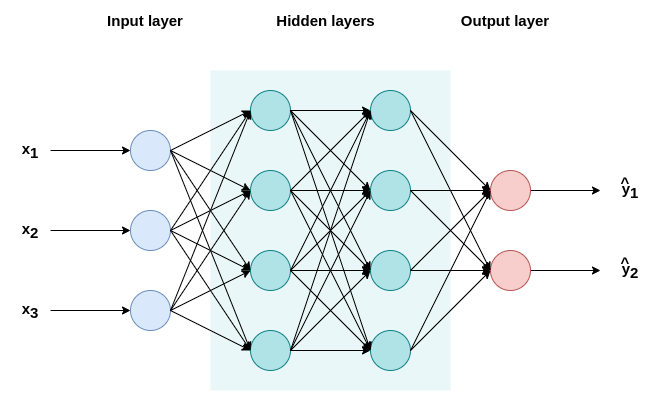
\includegraphics[width=0.7\linewidth]{images/background/neural_network.png}
	\caption[Artificial Neural Network]%
	{\textbf{Artificial Neural Network} with two hidden layers, $h_1$ and $h_2$, each consisting of a plethora of neurons.}
	\label{fig:neural_network}
\end{figure}

The neural network shown in the above figure is a Feedforward Neural Network (FFN), where the output of one layer is an input for the next layer. Each neuron of one layer is directly connected to all other neurons of the next layer. Due to this dense connectivity between neurons of each layer, such layers are called dense layers.

As Goodfellow et al. described in \cite{goodfellow}, the goal of a Feedforward Neural Network is to approximate some function $f^*$. According to the authors, It does so by defining a mapping $y = f(x;\theta)$ that maps the given input $x$ to a corresponding classification category $y$. The feedforward network learns the value of $\theta$ that returns the best function approximation.

The input layers accept the data from the outside world and transfer it directly to the first hidden layer without performing any computations.

Hidden layers are helpful when the linear separation of the data is not possible. Each neuron in a hidden layer is a perceptron that accepts inputs, computes a weighted sum (eq. \ref{eqn:weighted_sum}), applies the weighted sum to an activation function, and passes it towards the next layer.

The output layer of a neural network returns the final results based on the input it receives from its previous layer. The number of neurons in an output layer must match the expected outputs of its respective classification problem.  For example, if a neural network's task is to recognize the hand-written digits shown in figure \ref{fig:digits}, then the output layer of this neural network must have ten neurons where each neuron corresponds to a number from $0$ to $9$.

As with perceptron, neural networks also aim at minimizing the error. Due to the availability of hidden layers, the error is propagated backward using a chain rule, as explained in the following section.

\subsection{Backpropagation}\label{subsection:backprop}

Although the idea of backpropagation was initially pitched in the 1970s, it became famous by the work of Rumelhart et al. in \cite{backprop86} published in 1986. That paper showed the importance of this algorithm by demonstrating that it works better than other earlier approaches to learning. Given an error function for a neural network, the backpropagation algorithm computes the gradient of this error function. This computation happens backward, from the final layer to the first layer.

To properly understand how chain rule applies in error backpropagation, consider a simple neural network shown in below figure:

\begin{figure}[h]
	\centering
	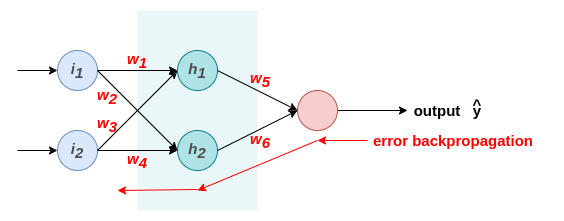
\includegraphics[width=0.7\linewidth]{images/background/back_prop.png}
	\caption[Backpropagation in a neural network]%
	{\textbf{Backpropagation} in a neural network with one hidden layer consisting of two hidden neurons $h_1$ and $h_2$, two input neurons $i_1$ and $i_2$, and one output.}
	\label{fig:back_prop}
\end{figure}

After getting output from the forward pass, we calculate the error using equation \ref{eq:error_func}. By using the partial derivative of this error, the following equation updates all the weights of the neural network:

\begin{equation}
    \label{eq:backprop_wu}
    w_j \coloneqq w_j - \eta \frac{\partial E}{\partial w_j}
\end{equation}

As stated before, we start error backpropagation from the final layer, i.e., the output layer of our neural network shown in figure \ref{fig:back_prop}. Consider the following figure that is visualizing the output layer of the neural network.

\begin{figure}[h]
	\centering
	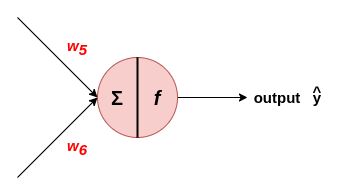
\includegraphics[width=0.4\linewidth]{images/background/back_prop_1.png}
	\caption[Backpropagating error from output layer]%
	{Backpropagating error from output layer to modify weights $w_5$ and $w_6$.}
	\label{fig:back_prop_1}
\end{figure}

To update $w_5$ and $w_6$, we must first compute $\frac{\partial E}{\partial w_5}$ and $\frac{\partial E}{\partial w_6}$. However, error $E$ is the difference between target $y$ and predicted output $\hat{y}$. Furthermore, the predicted output $\hat{y}$ is the result of applying the weighted sum to an activation function. Here, the weighted sum is calculated as:

\begin{equation}
    weighted\; sum\; (z) = \hat{y}_{h1} w_5 + \hat{y}_{h2} w_6
\end{equation}

where $\hat{y}_{h1}$ is output of the hidden neuron $h_1$ and $\hat{y}_{h2}$ is output of the hidden neuron $h_2$.

Based on this, we can derive the following formula that computes the partial derivative of $E$ with respect to $w_5$ and $w_6$ as:

\begin{equation}
    \frac{\partial E}{\partial w_5} = \frac{\partial E}{\partial \hat{y}} \frac{\partial \hat{y}}{\partial z} \frac{\partial z}{\partial w_5}
\end{equation}

\begin{equation}
    \frac{\partial E}{\partial w_6} = \frac{\partial E}{\partial \hat{y}} \frac{\partial \hat{y}}{\partial z} \frac{\partial z}{\partial w_6}
\end{equation}

We follow the similar process to compute the partial derivative of error $E$ with respect to $w_1$, $w_2$, $w_3$, and $w_4$.

Consider the following figure that is visualizing the hidden neuron $h_1$ of the neural network:
\begin{figure}[h]
	\centering
	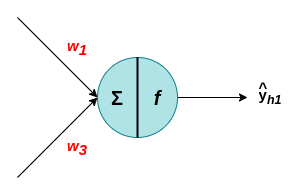
\includegraphics[width=0.4\linewidth]{images/background/back_prop_2.png}
	\caption[Backpropagating error from $h_1$]%
	{Backpropagating error from $h_1$ to modify weights $w_1$ and $w_3$.}
	\label{fig:back_prop_2}
\end{figure}

To update $w_1$ and $w_3$, we first compute $\frac{\partial E}{\partial w_1}$ and $\frac{\partial E}{\partial w_3}$ as:

\begin{equation}
    \frac{\partial E}{\partial w_1} = \frac{\partial E}{\partial \hat{y}_{h1}} \frac{\partial \hat{y}_{h1}}{\partial z_{h1}} \frac{\partial z_{h1}}{\partial w_1}
\end{equation}

\begin{equation}
    \frac{\partial E}{\partial w_3} = \frac{\partial E}{\partial \hat{y}_{h1}} \frac{\partial \hat{y}_{h1}}{\partial z_{h1}} \frac{\partial z_{h1}}{\partial w_3}
\end{equation}

Here, $\hat{y}_{h1}$ is output of the hidden neuron $h_1$ and $z_{h1}$ is the weighted sum used to compute $\hat{y}_{h1}$, calculated as:
\begin{equation}
    z_{h1} = i_1 w_1 + i_2 w_3
\end{equation}

Now, consider the following figure that is visualizing the hidden neuron $h_2$ of the neural network:
\begin{figure}[h]
	\centering
	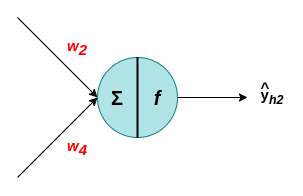
\includegraphics[width=0.4\linewidth]{images/background/back_prop_3.png}
	\caption[Backpropagating error from $h_2$]%
	{Backpropagating error from $h_2$ to modify weights $w_2$ and $w_4$.}
	\label{fig:back_prop_3}
\end{figure}

To update $w_2$ and $w_4$, we first compute $\frac{\partial E}{\partial w_2}$ and $\frac{\partial E}{\partial w_2}$ as:

\begin{equation}
    \frac{\partial E}{\partial w_2} = \frac{\partial E}{\partial \hat{y}_{h2}} \frac{\partial \hat{y}_{h2}}{\partial z_{h2}} \frac{\partial z_{h2}}{\partial w_2}
\end{equation}

\begin{equation}
    \frac{\partial E}{\partial w_4} = \frac{\partial E}{\partial \hat{y}_{h2}} \frac{\partial \hat{y}_{h2}}{\partial z_{h2}} \frac{\partial z_{h2}}{\partial w_4}
\end{equation}

Here, $\hat{y}_{h2}$ is output of the hidden neuron $h_2$ and $z_{h2}$ is the weighted sum used to compute $\hat{y}_{h2}$, calculated as:
\begin{equation}
    z_{h2} = i_1 w_2 + i_2 w_4
\end{equation}

Once we have the partial derivatives of error $E$ with respect to weights, we can use equation \ref{eq:backprop_wu} to update each weight, and then we train the neural network with updated weights. This process of weights update and re-training is repeated until the neural network converges.

Each layer in a traditional neural network is densely connected, making it a complex architecture. Also, in such a neural network, information travels only in the forward direction, i.e., there are no feedback loops available where the input to a function also depends on the output. However, there exist other variations of neural networks that are either computationally less complex (i.e., Convolutional Neural Networks) or support feedback loops (i.e., Recurrent Neural Networks).

A Convolutional Neural Network (CNN) ensures less computational complexity by forcing neurons of one layer to share weights. This sharing of weights reduces the number of learnable parameters, allowing for a better generalization. This process is based on the neocognitron network, published by K. Fukushima in \cite{neocognitronbc}. Results of \cite{7382560, 7822567} show that, in the areas of image recognition and classification, CNNs are very useful. However, similar to Feedforward Neural Networks, CNNs also do not have feedback loops. For this reason, Recurrent Neural Networks are better than CNNs while working on tasks where sequence order is essential such as machine translation or music composition.

% -----------------------------------------------------------------------------------------------------------
% ---------------------------------------- RECURRENT NEURAL NETWORKS ----------------------------------------
% -----------------------------------------------------------------------------------------------------------

\newpage
\section{Recurrent Neural Network}\label{section:rnn}

\begin{wrapfigure}{r}{6.4cm}
    \centering
    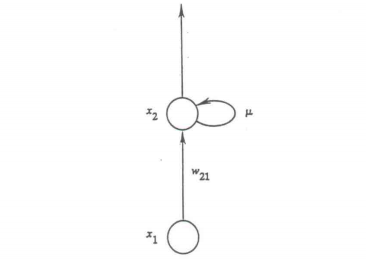
\includegraphics[width=1.0\linewidth]{images/background/jordan_rnn.png}
    \caption[A simple Recurrent Network]{A simple Recurrent Network as depicted in \cite{jordan}}
    \label{fig:jordan_rnn}
\end{wrapfigure} 

As stated before, one of the drawbacks of the standard neural network model is the lack of feedback loops. In 1986, M. Jordan published \cite{jordan}, in which he described Recurrent Networks as networks that have a connection from a unit to itself, i.e., a recurrent connection. This recurrent connection act as a feedback loop that makes it possible to use the previous outputs as inputs. This property of Recurrent Neural Networks makes them suitable to work with sequential information where all the inputs depend on each other.

As I. Sutskever describes in \cite{ilya}, a Recurrent Neural Network uses hidden states to incorporate new observations using an intricate nonlinear function. Such a Recurrent Neural Network can effortlessly be understated when it is unfolded in time, as shown in the figure:

\begin{figure}[h]
	\centering
	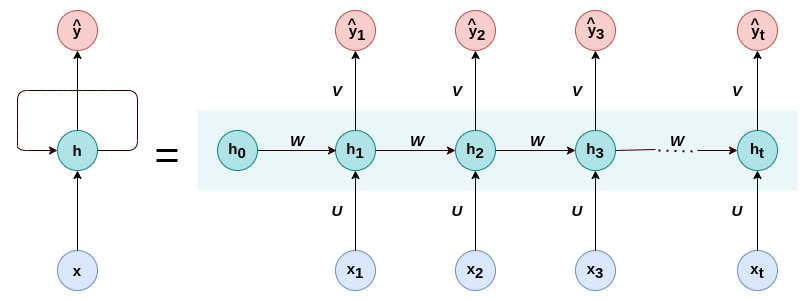
\includegraphics[width=0.9\linewidth]{images/background/rnn.png}
	\caption[A Recurrent Neural Network unfolded in time]%
	{A simple \textbf{Recurrent Neural Network} unfolded in time with $t$ sequences. Here, $U$ represents \textit{input-to-hidden weights}, $W$ represents \textit{hidden-to-hidden weights}, and $V$ represents \textit{hidden-to-output weights}.}
	\label{fig:rnn}
\end{figure}

The depicted Recurrent Neural Network accepts inputs $x_1, x_2, x_3, ..., x_t$, and outputs $\hat{y}_1, \hat{y}_2, \hat{y}_3, ..., \hat{y}_t$. The hidden states $h_0, h_1, h_2, h_3, ..., h_t$ are high-dimensional vectors, connected to each other to create recurrence. Deep extensions of a basic RNN can be constructed by stacking multiple recurrent hidden states on top of each other as shown in \cite{deeprnn}. Bias vectors $b_h$ and $b_o$, although are not shown in the above figure, are optional, but are useful to shift the activation function.

The RNN uses the following algorithm to compute $h_t$ and $\hat{y}_t$:

\begin{algorithm}
  \caption[Standard RNN algorithm]%
  {A standard RNN algorithm}
  \label{alg:rnn}
    \For{$t$ \textbf{from} $1$ \textbf{to} $T$}{
        \DontPrintSemicolon
        $z_{t} \gets U x_{t} + W h_{t-1} + b_{h}$ \tcp*{$b_{h}$ is optional}
        $h_{t} \gets e$($z_{t}$) \\
        $o_{t} \gets V h_{t} + b_{o}$ \tcp*{$b_{0}$ is optional}
        $\hat{y}_{t} \gets g$($o_{t}$)
    }
\end{algorithm}

where $e$($\cdot$) and $g$($\cdot$) are the hidden and output nonlinearities of the RNN. This computation of $h_t$ is visualized in the following figure:

\begin{figure}[h]
	\centering
	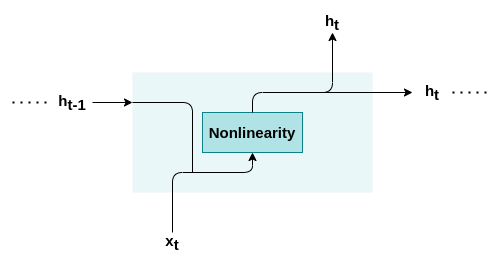
\includegraphics[width=0.6\linewidth]{images/background/rnn_unit.png}
	\caption[Internal structure of a single hidden unit in a standard RNN]%
	{The internal structure of a single hidden unit in a standard RNN visualizing the computation of $h_t$ using an input $x_t$, and the hidden state value of the previous unit $h_{t-1}$.}
	\label{fig:rnn_unit}
\end{figure}

The nonlinearity is required to produce a nonlinear decision boundary. Out of all three nonlinearities explained in section \ref{subsection:nonlinearity}, for the scope of this thesis, we only focus on ReLU and Tanh due to their added advantages over the Sigmoid activation function.

Similar to error backpropagation in traditional neural networks (as explained in section \ref{subsection:backprop}), RNNs also backpropagate error to update weights and minimize the absolute error. However, in recurrent networks, since the output of one time-step depends on previous ones, the error also backpropagates from time-step $t$ through the entire network to the first time-step. This is known as Backpropagation Through Time (BPTT \cite{bptt-1}).

\subsection{Backpropagation Through Time}\label{subsection:bptt}

To understand backpropagation through time, consider the following simple RNN with three time-steps visualizing error backpropagation from time-step 3:

\begin{figure}[h]
    \centering
    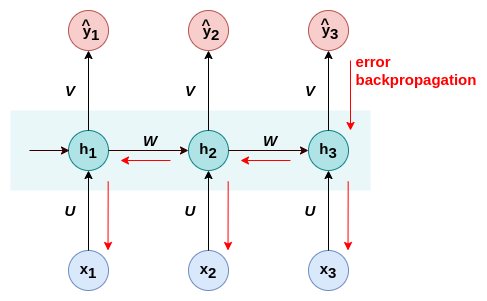
\includegraphics[width=0.7\linewidth]{images/background/bptt.png}
    \caption[Backpropagation Through Time]{A standard RNN visualizing BPTT from time-step 3. Here, $U$ represents \textit{input-to-hidden weights}, $W$ represents \textit{hidden-to-hidden weights}, and $V$ represents \textit{hidden-to-output weights}.}
    \label{fig:bptt}
\end{figure}

Error at time-step 3 $E_3$ is the difference between target output $y_3$  and predicted output $\hat{y}_3$. This error $E_3$ backpropagates from time-step 3 to time-step 1, as shown in the above figure. 

To start, using the algorithm \ref{alg:rnn}, we can write following equation for output $\hat{y}_3$:

\begin{equation}
    \hat{y}_3 = g(o_3)
\end{equation}

where $o_3$ is product of $V$ and $h_3$ given as:

\begin{equation}
    o_3 = V h_3
\end{equation}

where $V$ represents \textit{hidden-to-output} weights, $e$ is output nonlinearity, and $h_3$ is calculated as:

\begin{equation}
    h_3 = e(z_3)
\end{equation}

where, $z_3$ is the weighted sum computed as:

\begin{equation}
    \label{eq:z3}
    z_3 = Ux_3 + Wh_2
\end{equation}

where $U$ is \textit{input-to-hidden} weights, $W$ is \textit{hidden-to-hidden} weights, and $e$ is hidden nonlinearity.

As we can see in the above equations, to compute output $\hat{y}_3$, we need a total of three different weight vectors $V$, $W$, and $U$. Since our error $E_3$ is dependent on output $\hat{y}_3$, we must calculate the partial derivative of the error $E_3$ with respect to all three weight vectors, i.e., we need to compute $\frac{\partial E_3}{\partial V}$, $\frac{\partial E_3}{\partial W}$, and $\frac{\partial E_3}{\partial U}$. To compute these gradients, we follow the same chain rule as we did in backpropagation (section \ref{subsection:backprop}).

Calculating $\frac{\partial E_3}{\partial V}$ is easy as it only depends on $\hat{y}_3$, $o_3$. Therefore, by following the simple backpropagation, we can calculate $\frac{\partial E_3}{\partial V}$ as:

\begin{equation}
    \frac{\partial E_3}{\partial V} = \frac{\partial E_3}{\partial \hat{y}_3} \frac{\partial \hat{y}_3}{\partial o_3} \frac{\partial o_3}{\partial V}
\end{equation}

Calculation of $\frac{\partial E_3}{\partial W}$ is where calculation gets more complicated. To see why it is complicated from $\frac{\partial E_3}{\partial V}$, we first apply the chain rule as:

\begin{equation}
    \label{eq:wrt_W}
    \frac{\partial E_3}{\partial W} = \frac{\partial E_3}{\partial \hat{y}_3} \frac{\partial \hat{y}_3}{\partial h_3} \frac{\partial h_3}{\partial W}
\end{equation}

However, as we can see in equation \ref{eq:z3}, $z_3$ depends on $h_2$, which depends on $h_1$. For this reason, we cannot treat $h_2$ as constant; instead, we need to sum up the contributions of $h_2$ and $h_1$ as:

\begin{align}
    \frac{\partial h_3}{\partial W} &= \frac{\partial h_3}{\partial W} + \frac{\partial h_3}{\partial h_2} \frac{\partial h_2}{\partial W} + \frac{\partial h_3}{\partial h_2}\frac{\partial h_2}{\partial h_1}\frac{\partial h_1}{\partial W} \nonumber \\
                                    &= \frac{\partial h_3}{\partial h_3} \frac{\partial h_3}{\partial W} + \frac{\partial h_3}{\partial h_2} \frac{\partial h_2}{\partial W} + \frac{\partial h_3}{\partial h_1} \frac{\partial h_1}{\partial W} \nonumber \\
                                    &= \sum_{t=1}^{3} \frac{\partial h_3}{\partial h_t} \frac{\partial h_t}{\partial W} \label{eq:sum_h}
\end{align}

By substituting value from equation \ref{eq:sum_h} in equation \ref{eq:wrt_W}, we get

\begin{equation}
    \frac{\partial E_3}{\partial W} = \frac{\partial E_3}{\partial \hat{y}_3} \frac{\partial \hat{y}_3}{\partial h_3} \left[ \sum_{t=1}^{3} \frac{\partial h_3}{\partial h_t} \frac{\partial h_t}{\partial W} \right]
\end{equation}

We follow the similar process to calculate $\frac{\partial E_3}{\partial U}$ as:

\begin{equation}
    \frac{\partial E_3}{\partial U} = \frac{\partial E_3}{\partial \hat{y}_3} \frac{\partial \hat{y}_3}{\partial h_3} \left[ \sum_{t=1}^{3} \frac{\partial h_3}{\partial h_t} \frac{\partial h_t}{\partial U} \right]
\end{equation}

Similar to the backpropagation algorithm, we use these partial derivatives of error with respect to $V$, $W$, and $U$ to update the corresponding weights.

In standard RNNs, each hidden unit only performs the specified nonlinear activation (as depicted in figure \ref{fig:rnn_unit}). However, there exist other variations of RNNs, such as Long Short-Term Memory, Gated Recurrent Unit, that do more than just performing a single computation per hidden unit.

% -----------------------------------------------------------------------------------------------------------
% -------------------------------------------------- LSTM ---------------------------------------------------
% -----------------------------------------------------------------------------------------------------------

\newpage
\section{Long Short-Term Memory}\label{section:lstm}

Two of the problems with this algorithm are of exploding gradients\footnote{Exploding gradients is a problem when large error gradients accumulate, resulting in substantial updates to model weights making the model unstable.} or vanishing gradient\footnote{The vanishing gradient is a problem that prevents making changes in the weight values due to vanishingly small gradients.}. Two mitigate these problems, in 1997, Hochreiter et al. proposed a new recurrent architecture, termed Long Short-Term Memory (LSTM) in \cite{lstm}.

As opposed to the standard RNN's internal structure (figure \ref{fig:rnn_unit}), LSTM has a very different and much more complex internal structure made up of three gates (i.e., an \textit{input gate $i_t$}, an \textit{output gate $o_t$}, and a \textit{forget gate $f_t$}) to regulate the flow of information \cite{lstm_gates}. This is visualized in the following figure:

\begin{figure}[h]
	\centering
	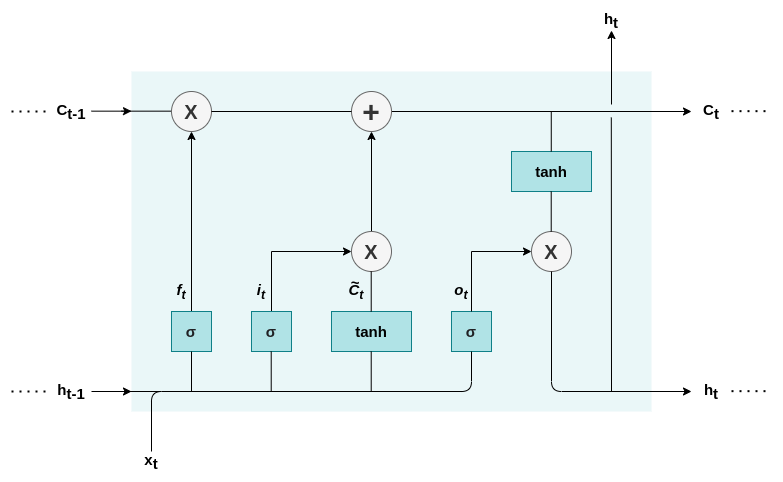
\includegraphics[width=0.8\linewidth]{images/background/lstm_unit.png}
	\caption[Internal structure of a single hidden unit in an LSTM]%
	{The internal structure of a single hidden unit in an LSTM visualizing the computation of $h_t$ and $C_t$ using an input $x_t$, the hidden state value of the previous unit $h_{t-1}$, and the cell state value of the previous unit $C_{t-1}$.}
	\label{fig:lstm_unit}
\end{figure}

Given an input $x_t$, previous hidden state $h_{t-1}$, and previous cell state $C_{t-1}$, the current hidden state $h_t$ and cell state $C_t$ can mathematically be calculated as follow:

\begin{enumerate}
    \item The first step is to compute the forget gate that informs the cell state about which past information to keep       and which one to forget.
        \begin{equation}
            \label{eqn:forget_gate}
            f_t = \sigma(W_f \cdot [h_{t-1}, x_t] + b_f)
        \end{equation}
        For each value in the cell state $C_{t-1}$, it returns a value between $0$ and $1$.
        
    \item The second step is to determine what new information needs to be stored in the cell state.
        \begin{equation}
            \label{eqn:input_gate}
            i_t = \sigma(W_i \cdot [h_{t-1}, x_t] + b_i)
        \end{equation}
        \begin{equation}
            \widetilde{C} _t = tanh(W_C \cdot [h_{t-1}, x_t] + b_C)
        \end{equation}
        The addition of these two values then will be used to update the previous cell state.
        
    \item The third step is to update the previous cell state as:
        \begin{equation}
            C_t = f_t * C_{t-1} + i_t * \widetilde{C}_t
        \end{equation}
        
    \item The final step is to compute the value for the output gate, that then will be used to update the hidden state       as:
        \begin{equation}
            \label{eqn:output_gate}
            o_t = \sigma(W_o \cdot [h_{t-1, x_t}] + b_o)
        \end{equation}
        \begin{equation}
            h_t = o_t * tanh(C_t)
        \end{equation}
    
    These updated state values, $h_t$, and $C_t$ are then forwarded to be used in the next unit.
\end{enumerate}

One of the benefits of LSTM over a standard RNN is the capability of learning long-term dependencies. Because of this added benefit, LSTMs have shown exceptional performance in many application areas including time series forecasting \cite{lstm_time}, drug design \cite{lstm_drug}, and music composition \cite{lstm_music}.

Although LSTMs have a better performance than standard RNNs, their execution is slower due to the availability of a higher number of computations. Therefore, another variation of RNNs, the Gated Recurrent Unit, is faster than an LSTM but has a better performance than a standard RNN.

% -----------------------------------------------------------------------------------------------------------
% --------------------------------------------------- GRU ---------------------------------------------------
% -----------------------------------------------------------------------------------------------------------

\newpage
\section{Gated Recurrent Unit}\label{section:gru}

The Gated Recurrent Unit (GRU) was introduced by Cho et al. in \cite{gru}. Similar to Long Short-Term Memory, Gated Recurrent Unit also aims to solve the vanishing gradient problem.

The internal structure of a GRU is very different from that of a standard RNN unit but is quite similar to that of an LSTM unit, except with only two gates (i.e., an \textit{update gate} $z_t$, and a \textit{reset gate} $r_t$) than three. These two gates control the flow of information that flows into and out of the memory \cite{gru_gates}. This internal structure is visualized in the following figure:

\begin{figure}[h]
	\centering
	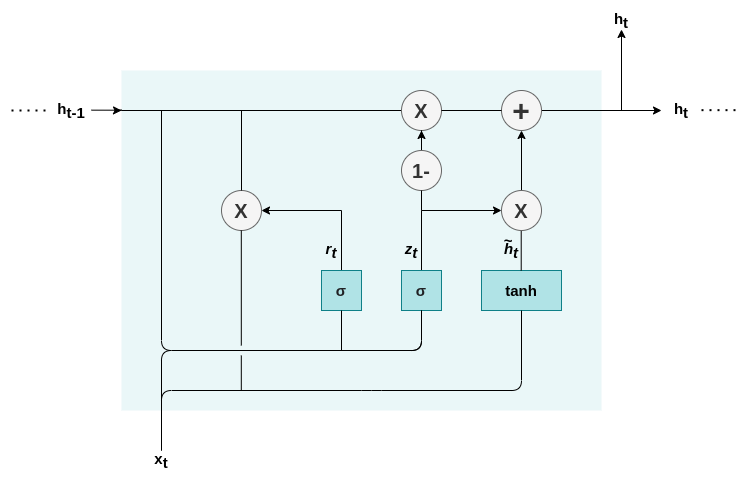
\includegraphics[width=0.8\linewidth]{images/background/gru_unit.png}
	\caption[Internal structure of a single hidden unit in a GRU]%
	{The internal structure of a single hidden unit in a GRU visualizing the computation of $h_t$ using an input $x_t$, and the hidden state value of the previous unit $h_{t-1}$.}
	\label{fig:gru_unit}
\end{figure}

Given an input $x_t$, and previous hidden state $h_{t-1}$, the current hidden state $h_t$ can mathematically be calculated as follow:

\begin{enumerate}
    \item The first step is to compute the update gate value as:
        \begin{equation}
            \label{eqn:update_gate}
            z_t = \sigma(W_z \cdot [h_{t-1}, x_t] + b_z)
        \end{equation}
        This gate helps to determine what information from the past to carry forward.
        
    \item The second step is to compute the value of the reset gate as:
        \begin{equation}
            \label{eqn:reset_gate}
            r_t = \sigma(W_r \cdot [h_{t-1}, x_t] + b_r)
        \end{equation}
        This gate decides how much of the past information to omit.
        
    \item The final step is to update the hidden state using the values of the update gate and the reset gate obtained        from equations \ref{eqn:update_gate} and \ref{eqn:reset_gate}, respectively.
        \begin{equation}
            \widetilde{h}_t = tanh(W_h \cdot [r_t * h_{t-1}, x_t] + b_h)
        \end{equation}
        \begin{equation}
            \label{eqn:update_hidden}
            h_t = (1 - z_t) * h_{t-1} + z_t * \widetilde{h}_t
        \end{equation}
        
    This updated hidden state value $h_t$ is then forwarded to be used in the next unit.
\end{enumerate}

Although LSTMs mostly outperform GRUs in many scenarios, GRUs have the upper hand when the dataset is small \cite{gru_lstm}. Similar to LSTM, GRUs are also capable of learning long-term dependencies. Because of this, GRUs have shown outstanding performance in different application areas, including speech recognition \cite{gru_speech} and water level prediction \cite{gru_water_level}.

In the scope of this thesis, we only focus on working with RNN with Tanh nonlinearity (RNN-Tanh), RNN with ReLU nonlinearity (RNN-ReLU), Long Short-Term Memory (LSTM), and Gated Recurrent Unit (GRU) as these four are the most popularly practiced recurrent networks.

% -----------------------------------------------------------------------------------------------------------
% ------------------------------------------------- PRUNING -------------------------------------------------
% -----------------------------------------------------------------------------------------------------------

\newpage
\section{Pruning}\label{section:pruning}

It is well known that the use of more extensive neural networks is favorable to achieve better performance, but at the same time, they are more expensive to use, takes more time to run, and in most cases, require expensive hardware. Therefore, in the past couple of decades, many researchers have worked on various model compression techniques to train large neural networks more efficiently while maintaining their accuracy. Pruning is one such technique that removes the top $k$ ranked weight parameters of a neural network. The weight parameters removed first are usually the ones with the most negligible impact on the model's final output.

In \cite{blalock}, Blalock et al. studied 81 different papers on pruning to identify important (hyper-)parameters and methods that give the best results with pruning compared to others. In that paper, the authors state that ``pruning methods vary primarily in their choices regarding sparsity structure, scoring, scheduling, and fine-tuning". Here, the sparse structure results from performing unstructured pruning in which individual weight parameters are pruned, and fine-tuning is the process of retraining the pruned neural network to identify the amount of pruning that can be applied without significantly reducing the performance.

There are different pruning techniques such as Magnitude-based pruning, Error-based pruning, Entropy-based pruning, Evolutionary pruning. In the scope of this thesis, we only focus on Magnitude-based pruning as it is proven to give satisfactory results despite being an easy technique.

\subsection{Magnitude-based pruning}

This is the simplest way of pruning that considers the magnitude of weight parameters as pruning criteria, meaning weight parameters that are least important are zeroed out before retraining the model to perform fine-tuning. Li et al. in \cite{li} state the OLMP (\textbf{O}ptimization based \textbf{L}ayer-wise \textbf{M}agnitude-based \textbf{P}runing) can reduce the size of AlexNet by 82\% without any loss inaccuracy. We also apply layer-wise pruning, where we first calculate threshold based on the percent of pruning to apply and zero-out values below this threshold using a binary mask.

% -----------------------------------------------------------------------------------------------------------
% ------------------------------------------------- GRAPHS --------------------------------------------------
% -----------------------------------------------------------------------------------------------------------

\newpage
\section{Graph Theory}\label{section:graphs}

Graph theory is the study of graphs, a network of nodes connected with edges. In \cite{carlson}, Carson states that the graph theory originated from Leonhard Euler's solution to the famous Königsberg bridge problem. This section briefly explores random graphs, their graph properties, and two random graphs with small-world properties, namely Watts–Strogatz and Barabási–Albert.

An undirected graph $G$ is given as a set of $(V, E)$, where $V$ is the set of nodes, and $E$, where $E \subseteq E_{comp} \coloneqq \{\{v, w\} | v, w \in V, v \neq w\}$ is the set of edges. A complete graph, $G_{comp}$, is a graph where each node is connected to every other node in the same network, which is different from a connected graph, where it is possible to get from one node to any other node in the same network via a series of edges.

Graphs, in mathematics, are usually used to model real-world structures, but if the structure is very complex and cannot model it in all details, random graphs are used.

\subsection{Random Graphs}\label{subsection:randomgraphs}

Random graphs, as the name states, have randomly distributed edges according to some probability measure. Based on which adequate probability measure is used, random graphs can be given as:

\begin{enumerate}
    \item \textbf{Uniform random graph}: For the given set of nodes $V$, edges $M$, and a probability space $\Omega$ where all graphs with nodes $V$ and $M$ edges has the uniform distribution, the probability is given as:
    \begin{equation}
        P(G) = \left( M_{comp} \atop M \right)^{-1}
    \end{equation}
    
    \item \textbf{Binomial random graph}: Given the probability $0 \leq p \leq 1$ that there exists an edge between two given nodes $v, w \in V$ and a probability space $\Omega$ where all graphs with nodes $V$ and edges $M$ has the binomial distribution, the probability is given as:
    \begin{equation}
        P(G) = p^M \cdot (1-p)^{M_{comp}-M}
    \end{equation}
\end{enumerate}

\subsection{Graph properties}\label{subsection:properties}

This section explores graph properties that we later use to find a correlation with performance. Along with simple properties such as the number of layers, the number of nodes, and the number of edges, we also use other graph properties, as given below:

\subsubsection{Diameter}
A graph's diameter is the maximal distance between any pair of nodes in a given graph, excluding any detours or loops. We can use the following equation to find the graph's diameter:
\begin{equation}
    \delta = \max_{ij}\{s(i, j)\}
\end{equation}
where $s(i,j)$ is the shortest path between two nodes $i$ and $j$.

\subsubsection{Density}
The density of a graph is the ratio of edges present to all possible edges. Given an undirected graph, the density of this graph is calculated as:
\begin{equation}
    d = \frac{2m}{n(n-1)}
\end{equation}
For a directed graph, the density is calculated as:
\begin{equation}
    d = \frac{m}{n(n-1)}
\end{equation}
where $n$ is the number of nodes, and $m$ is the number if edges.

\subsubsection{Average Shortest Path Length}
The average shortest path length is the mean number of steps on all potential pairs of nodes' shortest paths and is calculated as:
\begin{equation}
    a = \sum_{i,j \in V}\frac{d(i, j)}{n(n-1)}
\end{equation}
where $V$ is the set of nodes, $d(i,j)$ is the shortest path from node $i$ to $j$, and $n$ is the number of nodes.

\subsubsection{Eccentricity}
The eccentricity of a given node $V$ in a connected graph $G$ is the maximum distance from node $V$ to all other nodes in that graph. In contrast, for a disconnected graph, all nodes have an infinite eccentricity.

The maximum a graph can have is the graph diameter, while the minimum eccentricity is the graph radius.

\subsubsection{Degree}
The degree of a node is the number of nodes adjacent to that node.

\subsubsection{Closeness}
Closeness, often known as closeness centrality, indicates how close a node is to all other nodes in a given graph and is calculated as:
\begin{equation}
    C(u) = \frac{n-1}{\sum_{i=1}^{n=1}d(i, j)}
\end{equation}
where $d(i,j)$ is the shortest path between nodes $i$ and $j$, $n$ is the number of nodes in the graph.

\subsubsection{Node betweenness}
Node betweenness, also known as the betweenness centrality of node $u$, is the sum of the fraction of all shortest path pairs that pass through $u$ and is calculated as:
\begin{equation}
    c_B(u) = \sum_{i,j \in V}\frac{\sigma(i,j|u)}{\sigma(i,j)}
\end{equation}
Here, $V$ is the set of nodes, $\sigma(i,j)$ is the number of shortest paths between nodes $i$ and $j$, and $\sigma(i,j|u)$ is the number of shortest paths through node $u$.

\subsubsection{Edge betweenness}
In contrast to node betweenness, Edge betweenness is the number of shortest paths that pass through an edge in a given graph. It is calculated as:
\begin{equation}
    c_B(e) = \sum_{i,j \in V}\frac{\sigma(i,j|e)}{\sigma(i,j)}
\end{equation}
Here, $V$ is the set of nodes, $\sigma(i,j)$ is the number of shortest paths between nodes $i$ and $j$, and $\sigma(i,j|e)$ is the number of shortest paths through an edge $e$.

\subsection{Small World Networks}
In a Small World Network, the mean shortest-path distance between any two given nodes increases sufficiently slowly as a function of the number of nodes in the network \cite{porter}.

A Small World Network have the following three properties:
\begin{enumerate}
    \item \textbf{Higher order of the graph}: The order of a graph is simply the number of nodes in that graph, in other words, the cardinality of its node-set. In a Small World Network, the order of the graph is much higher than its average vertex degree.
    
    \item \textbf{Small characteristic path length}: As stated by F. Schreiber in \cite{schreiber}, the characteristic path length of a given graph is the average number of edges in the shortest paths between all pairs of nodes. For a given graph to be considered a Small World Network, it must have a small characteristic path length.
    
    \item \textbf{High clustering coefficient}: A clustering coefficient is a measure of the degree to which nodes in a graph are clustered together. A given graph must have a higher clustering coefficient to be considered a Small World Network.
\end{enumerate}

Watts–Strogatz is one of the popular Small World Networks, that is explained in the following section.

\subsubsection{Watts–Strogatz model}\label{subsubsection:wsmodel}
Watts–Strogatz (WS) are regular graphs with degree $k$. In 1998, Watts and Strogatz \cite{watts} proposed the Watts-Strogatz model to counteract the incomplete regularity and randomness in social networks.

The construction of a WS model begins with a lattice structure\footnote{A lattice graph is a graph embedded in a Euclidean space $\mathbb{R}$ that has a regular tiling form  \cite{lattice}.} that has a high clustering coefficient ($C$) but also a large characteristic path length ($L$). We can rewire some edges in this lattice structure to reduce $L$.

For each node $i \in V$, for each edge $\{i, j\}$ from node $i$ to one of the $r$ right neighbor $j$, the edge is left unchanged with probability $1-p$, and with probability $p$, the edge is replaced by a new edge $\{i, j\prime\}$ where $j\prime\in V \setminus (N(v) \cup \{v\})$ is randomly chosen.

For a small probability $p$, a sharp drop in characteristic path length ($L$) can be observed with no change in clustering coefficient ($C$).

\subsection{Scale Free Networks}\label{subsection:sfn}
In contrast to Small World Networks, where graphs have a small path length due to local clustering, Scale Free Networks have a skewed degree distribution \cite{aarstad}. Probability distribution of node degrees in such graphs is given as:
\begin{equation}
    P(d(v) = k) \sim k^{-\gamma}
\end{equation}
where $d(v)$ is the degree of node $v \in V$ and $\gamma$ is the power law factor.

As seen in the above equation, this probability distribution has power law where the probability of a node having a degree $k$ varies as the power law factor $\gamma$ varies.

In a Scale Free Network, the system grows with time, and new nodes and edges are added based on the preferential attachment. Such networks are observed in different science and technology areas such as the internet (nodes are HTML pages and edges are hyperlinks), electronic mail (nodes are email addresses and edges are sent emails between two users), and scientific literature (nodes are publications and edges are citations).

\subsubsection{Barabási–Albert model}\label{subsubsection:bamodel}
Barabási–Albert model is one of many Scale Free Networks that follows preferential attachment with power-law growth for a given system.

The construction of a Barabási–Albert model begins with $N_0 > 1$ nodes and $m < N_0$ edges where $N_0 = |V_0|$, cardinality of set of nodes at $t = 0$ without any edges.

At time $t = 1$, a new node is added to $V_0$ with $m$ edges from this new node to $m$ random different nodes.

At time $t > 1$, a new node is added to $V_{t-1}$ with $m$ edges from this new node to $m$ random different nodes, where the preferential attachment gives the probability of choosing node $i$ as:

\begin{equation}
    P(i) = c \cdot d(i)
\end{equation}
\centerline{where, $c = \frac{1}{\sum_{j \in V_{t-1}}d(j)}$}

In any given Barabási–Albert model, for any given time $t$, there are $N_0 + t = N_t$ nodes and $m \cdot t$ edges available.